\documentclass[11pt]{article}
\usepackage{colacl}
\usepackage[pdftex]{graphicx} 
\usepackage{booktabs}
\usepackage{tabularx}
\usepackage{pgfplots}
\usepackage{caption}
\usepackage{pgfplots}
\usepackage{rotating}
\usepackage{tikz}
\usepackage{float}
\usepackage[margin=1in]{geometry}
\usetikzlibrary{shapes.geometric, arrows}
\sloppy

\captionsetup[figure]{
    labelsep=period,
    justification=centering
}

\tikzstyle{startstop} = [rectangle, rounded corners, minimum width=3cm, minimum height=1cm, text centered, draw=black, fill=red!30]
\tikzstyle{io} = [trapezium, trapezium left angle=70, trapezium right angle=110, minimum width=3cm, minimum height=1cm, text centered, draw=black, fill=blue!30]
\tikzstyle{process} = [rectangle, minimum width=3cm, minimum height=1cm, text centered, draw=black, fill=orange!30]
\tikzstyle{arrow} = [thick,->,>=stealth]

\title{Exploring the impact of machine learning algorithms with unlabelled data}
\author
{Anonymous}



\begin{document}
\maketitle


%\begin{abstract}
%This is a \LaTeX\ sample for your paper.
%You shouldn't plan to include an abstract for a paper of this length.
%\end{abstract}

\section{Introduction}
Predicting salary based on job descriptions is a challenging task in the field of natural language processing and machine learning.
In the current digital age, many recruiters seek to find suitable candidates through multiple channels 
— e.g., online job portals, professional networks 
— as well as traditional avenues, such as word of mouth and mass media \cite{Primary-Organizational-Recruitment-Sources}.

The dataset is derived from the large dataset called \textit{mycareersfuture} \cite{bhola-etal-2020-retrieving}.
The dataset has a total of 17377 data, consisting of 13902 train data, 1738 validation data, and 1737 test data. 
The dataset is shown in the table \ref{tab:dataset_info}:


\begin{table}[h]
    \centering
    \caption{Dataset Information}
    \begin{tabular}{lrrr}
        \toprule
        Data Type      & Labeled & Unlabeled & Total \\
        \midrule
        Train          & 8000    & 5902      & 13902 \\
        Validation     & 1738    & -         & 1738  \\
        Test           & -       & 1737      & 1737  \\
        \midrule
        Total          & 9738    & 7639      & 17377 \\
        \bottomrule
    \end{tabular}
    \label{tab:dataset_info}
\end{table}

The distribution of salary bin is shown in the figure \ref{fig:dataset_output}.
We observe that the salary bin distribution exhibits an uneven and imbalanced pattern,
which may potentially affect the performance of the machine learning algorithms.


To answer the question "Does Unlabelled data improve Job salary prediction?", 
We will analyse and compare the performance of different machine learning algorithms for this dataset (labelled and unlabelled data) 
and finally explore whether unlabelled data can be effectively combined to increase the performance of the model.

\begin{figure}[t]
    \centering
    \includegraphics[width=0.5\textwidth]{dataset_output.png}
    \caption{Salary Bin Distribution}
    \label{fig:dataset_output}
\end{figure}

\section{Literature review}

In predicting salary based on job descriptions, there are many studies that have been conducted.
mycareersfuture dataset with job descriptions and their corresponding skills labels is presented by \cite{bhola-etal-2020-retrieving}.

Many methodology are proposed to predict salary based on job descriptions, such as BERT-XMLC \cite{bhola-etal-2020-retrieving}, 
framework for comprehensively evaluating the performance of debiasing methods \cite{han-etal-2022-systematic}.

Many traditional machine learning algorithms are also mentioned in this paper, 
such as kNN \cite{knn-Zhang2019/08}, 
Decision Tree \cite{dt_8718711}, 
Naive Bayes \cite{nb_10.1007/BFb0029444} and so on.



\section{Methods}

In this study, we adopt two feature representations from the raw job descriptions.

\begin{itemize}
    \item \textbf{TF-IDF}: We compute the TF-IDF vectors for job descriptions using the method proposed by \cite{manning2008introduction}. This method captures the importance of terms within a document and across the entire corpus.
    \item \textbf{Embedding}: We adopt the pretrained Sentence Transformer model \cite{reimers-gurevych-2019-sentence} to obtain word embeddings for the job descriptions. These embeddings provide semantic representation for the text data.
\end{itemize}


Through these two features, we explore three different machine learning algorithms paradigms: Supervised learning, Unsupervised learning and Semi-supervised learning.

To find the parameters which can lead the highest performance of the machine learning algorithms, we consider to use some search strategies.
Due to a high dimentions of the features, we adopt Grid search here because Grid search can suffer from high dimensional spaces \cite{liashchynskyi2019grid}.

We train the models between TFIDF and Embedding features, but we will only choose TFIDF features to analyse the results and evaluate the models.
To evaluate classifiers, we use the accuracy and $F_1$ score (\ref{eq:f1}) that combines recall (\ref{eq:recall}) and precision (\ref{eq:precision}) in the following way: \cite{TAN2006290}

\begin{equation}
    precision = \frac{TP}{TP + FP}
    \label{eq:precision}
\end{equation}

\begin{equation}
    recall = \frac{TP}{TP + FN}
    \label{eq:recall}
\end{equation}

\begin{equation}
    F_1 = 2 \times \frac{precision \times recall}{precision + recall}
    \label{eq:f1}
\end{equation}






% In the experiment, we decided to use salary bin as our target labels.
% To predict the salary bin, we will adopt the classification machine learning algorithms.
% We split our experiment into three parts: supervised learning, unsupervised learning, and semi-supervised learning.




\subsection{Supervised learning}
In the supervised learning part, we adopt 9 different machine learning algorithms to predict the salary bin.


\subsubsection{KNN Classifier}
We decide to use k-Nearest-Neighbours (kNN) as our baseline model, because the k-Nearest-Neighbours is a simple but effective method for classification \cite{10.1007/978-3-540-39964-3_62}.

To ensure what weights and p value in KNN classifier lead to a better performance,
we set the parameters of Grid search as follows:

\begin{itemize}
    \item \textbf{k}: 1 - 11
    \item \textbf{p}: 1, 2
    \item \textbf{weights}: uniform, distance
\end{itemize}

Using Grid search, we find that in TF-IDF, using kNN algorithm's best accuracy is 18.77\%.
In Embedding, using kNN algorithm's best accuracy is 23.95\%.
The best parameters are shown in the table \ref{tab:knn_results}.

\begin{table}[h]
    \centering
    \begin{tabularx}{0.45\textwidth}{@{}lcccc@{}}
    \toprule
    Features    & k & p & weights  & Accuracy    \\ \midrule
    TF-IDF         & 3 & 2 & distance  & 18.77  \\
    Embedding     & 3 & 2 & distance   & 23.95 \\ \bottomrule
    \end{tabularx}
    \caption{Best accuracies and parameters for kNN algorithm using TF-IDF and Embedding}
    \label{tab:knn_results}
\end{table}
    
    

In the experiment, we found that K is the most important factor in kNN algorithm. 
So we keep increasing k's value to 200.
And set p equal to 2 and weight is "distance". 
The output is shown in figure \ref{fig:knn}.

\begin{figure}[h]
    \centering
    \includegraphics[width=0.5\textwidth]{knn_output.png}
    \caption{KNN Classifier}
    \label{fig:knn}
\end{figure}


From the results, we can when the k value is 106, the accuracy for tfidf is 23.20\% which is the best accuracy for tfidf.
For embedding data, the best accuracy is 25.1\% when k is 26.


\subsubsection{Decision Tree Classifier}

Decision tree classifier is an effient supervised learning algorithm.
It focuses on generating classification rules displayed as decision trees that is deduced or concluded from a group of disorder and irregular instances. \cite{dt_8718711}
During the experiment, we adopted the decision tree classifier on the given dataset to see the performance.

We set 5 parameters during the experiment as follows:

\begin{itemize}
    \item \textbf{criterion}: gini, entropy
    \item \textbf{max\_depth}: 5, 10, 15
    \item \textbf{min\_samples\_split}: 2, 5, 10
    \item \textbf{min\_samples\_leaf}: 1, 2, 5
    \item \textbf{splitter}: best, random
\end{itemize}

After using Grid search, we find that in TF-IDF, using decision tree classifier's best accuracy is 20.38\%.
In embedding, using decision tree classifier's best accuracy is 18.77\%.
The best parameters are shown in the table \ref{tab:dt_results}.


\begin{table}[h]
    \centering
    \begin{tabularx}{0.5\textwidth}{@{}lcc@{}}
    \toprule
    Method     &  Parameters  & Accuracy \\ \midrule
    TF-IDF     & \begin{tabular}[t]{@{}l@{}}
                     criterion: gini \\
                     max\_depth: 15 \\
                     min\_samples\_split: 10 \\
                     min\_samples\_leaf: 2 \\
                     splitter: random
                   \end{tabular}  & 20.38 \\ \midrule
    Embedding  & \begin{tabular}[t]{@{}l@{}} 
                     criterion: entropy \\
                     max\_depth: 5 \\
                     min\_samples\_split: 2 \\
                     min\_samples\_leaf: 1 \\
                     splitter: random
                   \end{tabular} & 18.77  \\ \bottomrule
    \end{tabularx}
    \caption{Best accuracies and parameters for decision tree classifier using TF-IDF and Embedding}
    \label{tab:dt_results}
\end{table}
    


\subsubsection{Naive Bayes Classifier}

Naive Bayes \cite{nb_10.1007/BFb0029444} is a type of classifier based on probability.
We adopted two types of Naive Bayes classifier: BernoulliNB (\ref{eq:bernoulli}) and GaussianNB (\ref{eq:GaussianNB}).

\begin{equation}
    P(x_i|y) = P(x_i = 1 | y)x_i + (1 - P(x_i = 1 | y))(1 - x_i)
    \label{eq:bernoulli}
\end{equation}

\begin{equation}
    P(x_i|y) = \frac{1}{\sqrt{2\pi\sigma^2_y}} exp (-\frac{(x_i - \mu_y)^2}{2\sigma^2_y})
    \label{eq:GaussianNB}
\end{equation}



For naive Bayes classifier, we do not need to set parameters (as var\_smoothing does not influence a lot).
The accuracy is shown in the table \ref{tab:nb_results}.

\begin{table}[h!]
    \centering
    \caption{Accuracy of Naive Bayes Models}
    \label{tab:nb_results}
    \begin{tabular}{lcc}
    \toprule
    \textbf{Model} & \textbf{TF-IDF} & \textbf{EMD} \\
    \midrule
    GaussianNB     & 21.99 & 22.91 \\
    BernoulliNB    & 21.47 & 21.3 \\
    \bottomrule
    \end{tabular}
\end{table}

From the table \ref{tab:nb_results}, we can see that the accuracy of GaussianNB is higher than BernoulliNB.

\subsubsection{Other Classifier}

In the experiment, we also tried other supervised classifiers such as SVM \cite{svm_rejani2009early}, Adaboost and some ensemble methods.
The results are shown in the table \ref{tab:all_results}.
Of these, the SVM model got the best accuracy of 26.89\% in embedding features.

\subsection{Unsupervised learning}

Due to there has many unlabeled data in the dataset,
we also tried to use unsupervised learning to train the model.
However, the result is unsatisfactory.

In the experiment, we used K-means clusting algorithm and Gaussian mixture model (GMM) algorithm to train the model.
The accuracy is shown in the table \ref{tab:unsupervised_results}.

\begin{table}[h!]
    \centering
    \caption{Accuracy of Unsupervised Models}
    \label{tab:unsupervised_results}
    \begin{tabular}{lcc}
    \toprule
    \textbf{Model} & \textbf{TF-IDF} & \textbf{Embedding} \\
    \midrule
    K-means & 15.66 & 16.41 \\
    GMM     & 11.23 & 11.51 \\
    \bottomrule
    \end{tabular}
\end{table}

\begin{figure}[t]
    \centering
    \includegraphics[width=0.5\textwidth]{Self-trained-semi-supervised-learning-architecture.png}
    \caption{Self-trained semi-supervised learning architecture \cite{Self-trained-semi-supervised-learning}}
    \label{fig:Self-trained}
\end{figure}

\subsection{Semi-supervised learning}

For semi-supervised learning, we adopted self-training method \cite{Self-trained-semi-supervised-learning}.
The architecture is shown in figure \ref{fig:Self-trained}.



\begin{table*}[h]
    \centering
    \caption{$F_1$ scores of all models}
    \begin{tabularx}{\textwidth}{|l|X|X|X|X|}
    \hline
    \textbf{Method} & \multicolumn{2}{c|}{\textbf{Supervised}} & \multicolumn{2}{c|}{\textbf{Semi-supervised}} \\ \cline{2-5}
                    & \textbf{TF-IDF} & \textbf{Emb} & \textbf{TF-IDF} & \textbf{Emb} \\ \hline
    KNN             & 0.2118          & 0.2108       & 0.1042          & 0.2194       \\
    DT              & 0.1602          & 0.1678       & 0.1377          & 0.1597       \\
    GNB             & 0.1994          & 0.2082       & 0.1884          & 0.2114       \\
    BNB             & 0.1778          & 0.1908       & 0.1761          & 0.2038       \\
    Adaboost        & 0.1765          & 0.1651       & 0.1880          & 0.1779       \\
    DT+Adaboost     & 0.2116          & 0.1934       & 0.1849          & 0.1905       \\
    GNB+Adaboost    & 0.1911          & 0.1605       & 0.1154          & 0.1263       \\
    SVM             & \textbf{0.2466}$^*$  & \textbf{0.2616}$^*$       & \textbf{0.2333}$^*$          & \textbf{0.2389} $^*$        \\ \hline
    \end{tabularx}
    \label{tab:f1_results}
\end{table*}

\begin{table*}
    \begin{center}
        \captionof{table}{Accuracy of all models} \label{tab:all_results}
        \begin{tabularx}{\textwidth}{@{}l *{7}{>{\centering\arraybackslash}X} @{}}
        \toprule
        Model & \multicolumn{2}{c}{TFIDF} & \multicolumn{2}{c}{Embedding}\\
        \cmidrule(lr){2-3} \cmidrule(lr){4-5}
        & Labaled data & Unlabeled data & Labaled data & Unlabaled data \\
        \midrule
        
        	KNN & 18.77 & 20.21 & 23.95 & 25.1 \\
        	GNB & 21.99 & 21.12 & 22.91 & 21.99 \\
        	BNB  & 21.47 & 20.43 & 21.3 & 20.84 \\
        	Adaboost & 22.39 & 20.43 & 21.7 & 19.8 \\
        	Decision Tree (DT) & 20.38 & 20.03   & 16.29 & 17.9 \\
        	Adaboost + DT & 22.22 & 19.86 & 21.7 & 23.2 \\
        	Adaboost + GNB & 21.99 & 10.99 & 17.67 & 13.82 \\
        	Adaboost + BNB & 22.51 & 10.99 & 21.53 & 14.91 \\
        	SVM & \textbf{25.62}$^*$ & \textbf{24.64}$^*$ & \textbf{26.89}$^*$ & \textbf{24.87}$^*$ \\
        	\cmidrule(lr){1-5} 
        	K-means & - & \textbf{15.66}$^*$ & - & \textbf{16.41}$^*$ \\
        	GMM & - & 11.23 & - & 11.51 \\
        
        \bottomrule
        \end{tabularx}
        \caption*{Note: The ublabeled data of supervised learning means using the self-training method.}
    \end{center}
\end{table*}

The method of self-training is to use the labeled data to train the model,
and then use the trained model to predict the unlabeled data's label.
If the probability of the predicted label is greater than the threshold, 
then we add the unlabeled data with its predicted labels to the training set and retrain the model.

On the basis of this, we using the unlabeled data by iteratively training the model and selecting the high-confidence (greater than the threshold).
We set two conditions for stopping the iteration:

\begin{itemize}
    \item There is no high-confidence samples in the unlabeled dataset.
          (high-confidence means the probability of the predicted label is greater than the threshold)

    \item There is no improvement after iterations. 
          The moethod keep tracking the best accuracy that is achieved by the model on the validation set.
          If the accuracy does not improve of 3 iterations, the method will stop.
          This helps avoid the overfitting and saves compute resources and time.
\end{itemize}

The goal is to improve the performance of the model by using the unlabeled data.

In the experiment, we define two self-trained models, one with the threshold as 0.8, and one without threshold.
We dicover that self-trained model can not improve the performance of the model.
The accuracy is shown in the table \ref{tab:all_results}.

We discover that the self-trained method can not improve much performance of the model, 
some accuracy have even decreased.


\begin{figure*}
    \centering
    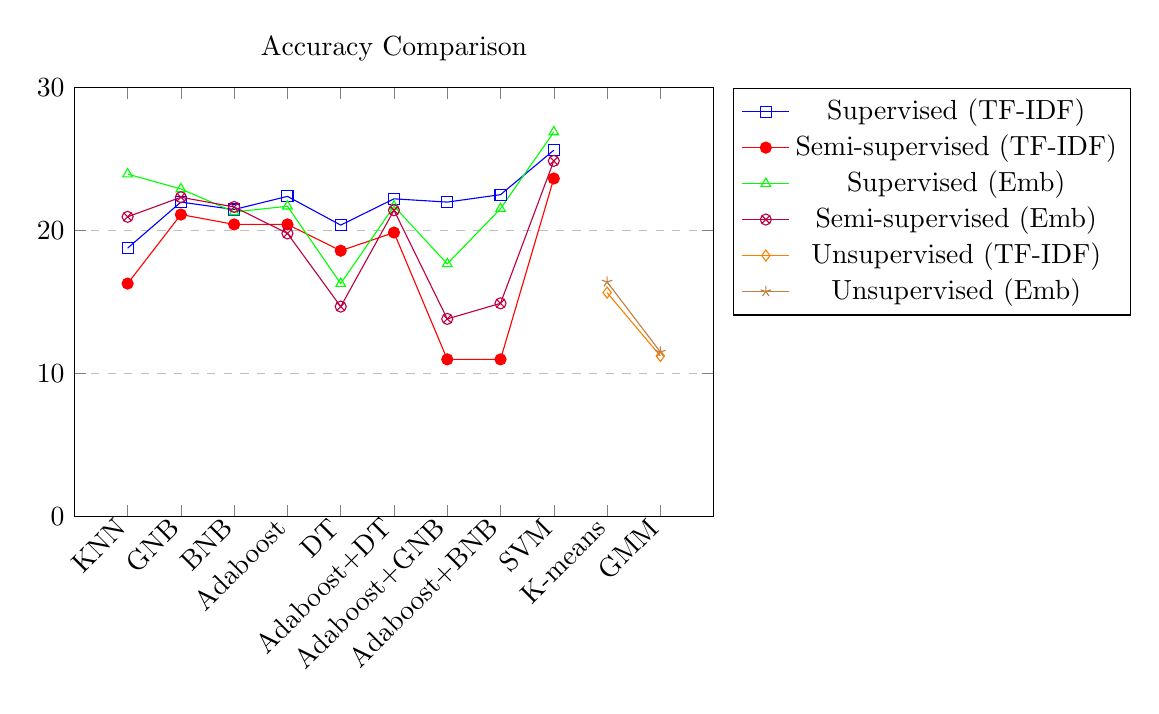
\begin{tikzpicture}
        \begin{axis}[
            title={Accuracy Comparison},
            % xlabel={Models},
            % ylabel={Accuracy},
            xmin=0, xmax=12,
            ymin=0, ymax=30,
            xtick={1, 2, 3, 4, 5, 6, 7, 8, 9, 10, 11, 12},
            xticklabels={
                KNN, GNB, BNB, Adaboost, DT, Adaboost+DT, Adaboost+GNB, Adaboost+BNB, SVM, K-means, GMM},
            xticklabel style={rotate=45, anchor=east},
            legend pos=outer north east,
            ymajorgrids=true,
            grid style=dashed,
            width=0.8\textwidth,
            height=200,
        ]
    
        % Labeled data (TFIDF)
        \addplot[
            color=blue,
            mark=square,
        ]
        coordinates {
            (1,18.77) (2,21.99) (3,21.47) (4,22.39) (5,20.38) (6,22.22) (7,21.99) (8,22.51) (9,25.62)
        };
        \addlegendentry{Supervised (TF-IDF)}
        
        % Unlabeled data (TFIDF)
        \addplot[
            color=red,
            mark=*,
        ]
        coordinates {
            (1,16.29) (2,21.12) (3,20.43) (4,20.43) (5,18.59) (6,19.86) (7,10.99) (8,10.99) (9,23.64)
        };
        \addlegendentry{Semi-supervised (TF-IDF)}
        
        % Labeled data (Embedding)
        \addplot[
            color=green,
            mark=triangle,
        ]
        coordinates {
            (1,23.95) (2,22.91) (3,21.3) (4,21.7) (5,16.29) (6,21.7) (7,17.67) (8,21.53) (9,26.89)
        };
        \addlegendentry{Supervised (Emb)}
    
        % Unlabeled data (Embedding) - Semi-supervised
        \addplot[
            color=purple,
            mark=otimes,
        ]
        coordinates {
            (1,20.96) (2,22.33) (3,21.65) (4,19.8) (5,14.68) (6,21.42) (7,13.82) (8,14.91) (9,24.87)
        };
        \addlegendentry{Semi-supervised (Emb)}
        
        % Unlabeled data (Embedding)
        \addplot[
            color=orange,
            mark=diamond,
        ]
        coordinates {
            (10,15.66) (11,11.23)
        };
        \addlegendentry{Unsupervised (TF-IDF)}

        \addplot[
            color=brown,
            mark=star,
        ]
        coordinates {
            (10,16.41) (11,11.51)
        };
        \addlegendentry{Unsupervised (Emb)}
        
        \end{axis}
    \end{tikzpicture}
    \caption*{}
    \label{fig:all_acc_results}
\end{figure*}


\section{Results}

In this section, we present the results of our experiments.
We evaluate the performance of our models by using the $F_1$ score and accuracy.
The results which shown in the table \ref{tab:all_results} and table \ref{tab:f1_results} are the results of models with best parameters after adopting grid search.

Table \ref{tab:f1_results} shows the $F_1$ scores of all models,
and table \ref{tab:all_results} shows the accuracy of all models.



In the experiment, we adopt the wandb to record the our runs results.
The detailed results of the experiment will be published in the wandb reporepository \footnote{Due to it is anonymous, it can not be shown now.}.




\section{Discussion}

In this study, we explore the performance of various machine learning models on the task of predicting salary based on job descriptions using
supervised, unsupervised and semi-supervised learning algorithms.

Our result indicate that the overall performance of the models is not satisfactory,
with approximately 20\% for most models.
Among the models, we find that the SVM model got the best accuracy of 26.89\% and the best $F_1$ score 0.2616.

In semi-supervised learning, we observe that the incorporation of unlabeled data using trained model does not consistently improve the performance.
After checking the predicted probabilities generated by the predict\_proba method in scikit-learn,
we find that the probability of the predicted labels do not have a high probability (most of them are below 0.4).
As a result, when we add all the unlabled data with its predicted labels to the training set,
the data who has a low probability sometimes get an incorrect predicted label.
This is a reason that make the accuracy and $F_1$ score decrease.


To address this probelm, We explore the possibility of setting a threshold to filter out instances with low probability estimates.
following the approach proposed by \cite{Self-trained-semi-supervised-learning}.
By iteratively training the model and selecting the high-confidence (greater than the threshold) unlabeled data,
which is effiently reduce the impact of low-confidence values.
However, it still can not lead a better performance to the models.

This suggests that the self-training method with a confidence threshold can not use unlabelled data to improve the performance of the model in this task.
I think the further optimization of the model parameters and the feature engineering of the data may be helpful to improve the performance of the model.



\section{Conclusions}

In conclusion, our study demonstrates that the challenges in leveraging unlabeled data to improve the performance of the model.
The SVM model achieved the best performance in this task but the overall accuracy and $F_1$ score remains low.
Furthermore, the self-training method with confidence threshold does not consistently improve the performance of the models,
which suggests that the further research and optimization in semi-supervised learning methods for this task is needed.





\nocite{*}
\bibliographystyle{apalike}
\bibliography{sample}

\end{document}
